%初版作者:2018级信息与计算科学张奥星
%本版作者:2019级数学与应用数学朱鹏宇
%有关于模板的疑问可以咨询qq:1760591167


%%%%%%%%%导言区%%%%%%%%%%%%%%
%自定义的文档类
\documentclass{hainanuthesis}
%一些常用宏包
\usepackage{amsthm,amsfonts,color,tikz,mathrsfs,hyperref,float,subfig,booktabs,listings}

%插入网址链接
\hypersetup{hidelinks,
	colorlinks=true,
	allcolors=black,
	pdfstartview=Fit,
	breaklinks=true}

%%%%%%%参考文献设置%%%%%%%%%%
%参考文献宏包
\usepackage[backend=bibtex,style=gb7714-2015]{biblatex}
%参考文献字体格式
\renewcommand\bibfont{\zihao{5}}
%导入参考文献bibtex文件
\addbibresource{ref.bib}

%定义定理格式环境
\theoremstyle{definition}
\newtheorem{theorem}{\indent 定理}[section]
\newtheorem{lemma}[theorem]{\indent 引理}
\newtheorem{proposition}[theorem]{\indent 命题}
\newtheorem{corollary}[theorem]{\indent 推论}
\newtheorem{definition}{\indent 定义}[section]
\newtheorem{example}{\indent Example}[section]
\newtheorem{remark}{\indent 注}[section]
\newenvironment{solution}{\begin{proof}[\indent\bf 解]}{\end{proof}}
\renewcommand{\proofname}{\indent\bf 证明}


%%%%%%%%%%%%%导言区%%%%%%%%%%%%%%%%%%

\title{海南大学毕业设计模板}
\author{xxx}
\id{123456789}
\grade{20xx级}
\faculty{x学院}
\department{x系}
\major{xxxx}
\teacher{xxx}


\begin{document}
	%创建封面
	\makecover
	%%%%%%%%%%摘要%%%%%%%%%%%%
	\begin{abstract}
		这是中文摘要
		\keywords{中文;关键字}
	\end{abstract}

	%该页面不显示页码
	\thispagestyle{empty}
	
	%换页	
	\newpage
	\begin{abstract}[en]
		This is English abstracts.
		\keywords[en]{English; Keywords}
	\end{abstract}
	\thispagestyle{empty}
	
	%%%%%%%%%%目录%%%%%%%%%%%%%
	\newpage
	\tableofcontents
	%目录页不参与页码计数
	\thispagestyle{empty}
	
	%%%%%%%%%%%%正文%%%%%%%%%%%
	\newpage
	%从此页码开始,从页码1开始计数
	\setcounter{page}{1}
	\section{介绍}
	
	本模板在2018级信息与计算科学专业学长制作的模板\footnote{https://github.com/OdinZhang/hainanuthesis}基础上,结合笔者自身毕业论文使用经验进行了修正和内容补充,更适用于理工科尤其是数学、物理等专业的学生的使用。
	
	\LaTeX 可以让写作者更加关注文章的内容而非格式,并且在数学公式的编写上更具优势(基于tikz宏包,使用\LaTeX 也可以比较方便地创作一些数学图形)。如果读者没有使用\LaTeX 的经验,建议读者阅读lshort文档\footnote{\href{https://www.ctan.org/pkg/lshort-zh-cn}{https://www.ctan.org/pkg/lshort-zh-cn}}以及刘海洋\cite{liuhaiyang2013}编写的《\LaTeX 入门》。前者作为最经典的\LaTeX 使用手册,浅花一段时间进行浏览和实践能够让你对\LaTeX 有一个比较清晰的认识。后者比较厚,是一本书,适合进行深入学习。事实上,笔者对本模板的进行完善补充的知识大多是从这两个资料中获得的。
	
	文中会对一些可能用的到的命令做简要说明,事实上其中大部分都可以在书中或者网络上搜集到相关知识。如果有其他疑问请联系作者。学长已经工作也许比较忙,直接联系我即可。
	
	本模板目前只是初版,笔者自身水平有限,难免有疏漏或者不规范的地方欢迎与笔者交流。后续模板维护将更新在我的主页上\footnote{\href{https://nalydz.github.io/}{https://nalydz.github.io}}。
	
	\subsection{使用的宏包}

	本模板目前所使用的宏包见\cref{tb:01}。
	
	\begin{table}[H]
		\begin{center}
			\caption{宏包及功能}
			\label{tb:01}
			\begin{tabular}{llll}
				\verb|fontspec| & 英文字体设置           &\verb|amsthm  | & 支持定理格式的切换\\
				\verb|expl3   | & \LaTeX 3语法设置       &\verb|amsfonts| & 丰富的数学符号    \\
				\verb|hyperref| & 启用文章超链接及PDF书签 &\verb|color   | & 对颜色进行支持   \\
				\verb|geometry| & 页面布局设置           &\verb|tikz    |& 支持一些绘图功能   \\
				\verb|fancyhdr| & 页眉页脚设置           &\verb|mathrsfs|& 花体大写字母       \\
				\verb|titletoc| & 目录格式设置           &\verb|float   |& 为浮动体提供H位置参数\\
				\verb|cleveref| & 公式、图片、表格等的引用&\verb|subfig  | & 图片定义小标题 \\
				\verb|caption | & 公式、图片、表格等的标号&\verb|booktabs| & 支持三线表  \\
				\verb|biblatex| & 参考文献的引用   &\verb|listings| & 生成高亮代码环境     \\
			\end{tabular}
		\end{center}
	\end{table}
	
	\subsection{编译}
	
	\begin{verbatim}
		latexmk
		-synctex=1
		-interaction=nonstopmode
		-file-line-error
		-pdf
		-xelatex
		main.tex
	\end{verbatim}
	
	\subsection{TeXlive+TeXstudio}
	
	本模板在TeXlive+TeXstudio环境下运行正常,事实上这也是比较推荐的运行方式。相关下载安装可以参考文档Install-LaTeX-Guide-zh-cn \footnote{\href{https://github.com/OsbertWang/install-latex-guide-zh-cn}{https://github.com/OsbertWang/install-latex-guide-zh-cn}}。
	
	国内有关于\LaTeX 的问答网站\footnote{\href{https://ask.latexstudio.net}{https://ask.latexstudio.net}},请一定注意提问时提供最小工作示例。该网站的主站\footnote{\href{https://www.latexstudio.net}{https://www.latexstudio.net}}有大量的\LaTeX 模板,包括数学建模国赛模板等。该网站相关QQ群号码为:91940767,也可进群提问,里面会解答什么是最小工作示例。
	
	\LaTeX 也有线上运行方式,方便线上编写以及多人协作,如overleaf \footnote{\href{https://www.overleaf.com/}{https://www.overleaf.com/}},最近貌似有了国产线上版本TexPage\footnote{\href{https://texpage.com/}{https://texpage.com/}}。不过友情提示,涉及隐私的东西尽量选择在本地进行哦。
	
	\section{部分命令演示}
	
	模板中用到的命令基本都有注释,下面做一些其他补充说明。
	\subsection{封面}
	
	使用命令
	\verb|\makecover|
	来创建一个新的封面。
	
	封面设置中新定义的命令与实际含义的对应关系见\cref{tb:02}。
	
	\begin{table}[!htbp]
		\begin{center}
			\caption{命令及含义}
			\label{tb:02}
			\begin{tabular}{ll}
				\verb|\id|         & 学号     \\
				\verb|\grade|      & 年级     \\
				\verb|\faculty|    & 学院     \\
				\verb|\department| & 系别     \\
				\verb|\major|      & 专业     \\
				\verb|\teacher|    & 指导老师 \\
			\end{tabular}
		\end{center}
	\end{table}
	
	\subsection{摘要与关键字}
	
	\subsubsection{摘要}
	\begin{verbatim}
		\begin{abstract}
			
		\end{abstract}
	\end{verbatim}
	
	上述命令将显示中文摘要。
	
	\begin{verbatim}
		\begin{abstract}[en]
			
		\end{abstract}
	\end{verbatim}
	
	上述命令将显示英文摘要。
	其中中括号中内容不为\verb|zh|时均为英文。
	
	\subsubsection{关键字}
	
	中文关键字为\verb|\keywords{}|,
	英文关键字为\verb|\keywords[en]{}|。
	同样的,
	中括号内参数不为\verb|zh|时均为英文。
	
	\subsection{三线表}
	
	科技论文中经常需要使用到三线表,\cref{tb:03}是一个示例。表格的一些自定义方法见lshort。
	\begin{table}[H]
		\caption{三线表示例}
		\centering
		\label{tb:03}
		\setlength{\tabcolsep}{3pt}
		\begin{tabular}{ccccccc}
			\toprule[1.5pt]
			来源 & SS & df & MS & F & P & F-crit \\
			\midrule[1pt]
			组间 & 4.2733 & 1 & 4.2733 & 69.5978 & 2.91739E-13 & 3.93\\
			组内 & 6.5083 & 106 & 0.0613 & & &\\
			总计 & 10.7816 & 107 &  & & & \\
			\bottomrule[1.5pt]
		\end{tabular}
	\end{table}
    
    \subsection{基于tikz画图}
	tikz宏包提供了一些画图命令,\cref{pt:01}是一个交换图的例子。熟练使用tikz可以画更复杂、更美观的图形,可以结合有关资料自己摸索,这需要一些时间。如果任务紧集,建议直接插图。此外,对比观察图、表标题,不难发现图表标题的位置与\verb|\caption{}|命令的位置有关。
	\begin{figure}[H]
		\centering
		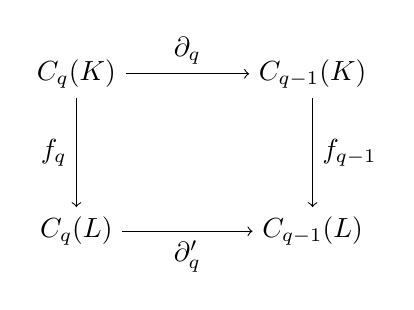
\begin{tikzpicture}
			\node (a) at (-1.5, 1) {\(C_q(K)\)};
			\node (b) at (1.5, 1) {\(C_{q-1}(K)\)};
			\node (c) at (-1.5, -1) {\(C_q(L)\)};
			\node (d) at (1.5, -1) {\(C_{q-1}(L)\)};
			\draw[->] (a) -- (b) node[midway, above] {\(\partial_q\)};
			\draw[->] (a) -- (c) node[midway, left] {\(f_q\)};
			\draw[->] (c) -- (d) node[midway, below] {\(\partial_q^\prime\)};
			\draw[->] (b) -- (d) node[midway, right] {\(f_{q-1}\)};
		\end{tikzpicture}
		\caption{交换图}
		\label{pt:01}
	\end{figure}
	
	\subsection{多行公式}
	
	多行公式的排版同样参考lshort即可,类似分段函数的多行公式可以参考以下示例。
	
	\[\partial s^q = \left\{
		\begin{array}{ll}
			0, & q=0,\\
			\sum\limits_{i=0}^q(-1)^i a_0\cdots \hat{a_i}\cdots a_q, &  q = 1,\dots \mathop{dim}~K,
		\end{array} \right. 
	\]
	
	其他\LaTeX 命令与功能(如浮动体、字体、数学公式等)在lshort等资料中均有详细介绍,就不再多赘述了。关于页面格式,本模板没有提供左侧装订线,可以在打印时调节。
	
	\subsection{参考文献}
	
	参考文献相关命令已由\verb|\reference|封装好,只需将导出的\verb|biblatex|格式文本保存到\verb|ref.bib|文件夹即可。
	如果想要更改,可以对hainanuthesis.cls文档类文件进行操作。
	\subsection{致谢}
	插入相关环境即可,见模板自身示例。
	
	
	
	\subsection{附件}
	
	插入\verb|\addons|命令即可,见模板自身示例。
	
	
	\newpage
	\begin{acknowledge}
		文档写到这里,就算告一段落了。再一次看到大大的“致谢”两个字,临近毕业,突然又想说点什么。
		
		为什么会想到做这样一个模板呢?也许是自己想留下什么痕迹的愿望。本科在海大呆了四年,临别前做点事情也不错。下午看书的时候想起这件事情,立马就行动起来。说来也怪,相比写毕设时调格式的磕磕绊绊,这次的完善工作居然出奇地顺利。
		
		也许下一届使用这个模板的学弟学妹我还认得,再过几年,如果模板还能流传下去,那素未谋面的我们在这一时刻就产生了奇妙的联系。我不太能表达心里的感觉,前些天院长说要成立数学统计学院了,想到这里,更觉得这好像是一种传递。也是在最近,我发现了18级学长关于飞跃手册的工作。我很喜欢这个项目,主动联系了负责人,希望能做点贡献,让手册的内容丰富起来,可以持续下去。
		
		算了,不矫情啦。祝海南大学越来越好,祝海大数学学科越来越好,希望我们,也越来越好。
	\end{acknowledge}
	
	%参考文献部分
	\newpage
	\reference
	
	\newpage
	\addons
	这里是附件部分。
	
	
	
	
\end{document}